\chapterbegin{Introducción al ensamblador}
\label{chp:IntrEnsam}
\minitoc

{\bf Objetivo}:
En esta sesión vamos a conocer el entorno de trabajo.
Veremos qué aspecto tiene un programa en ensamblador, veremos cómo
funcionan los tres programas que vamos a utilizar: el ensamblador,
el {\it enlazador (linker)} y el {\it depurador (debugger)}.
Del {\it debugger} sólo mostraremos unos pocos comandos,
que ampliaremos en las próximas sesiones.
También veremos la representación de los números naturales y de los
enteros, y el funcionamiento de algunas de las instrucciones del ARM.
Se repasarán también los conceptos de registros, flags e instrucciones
para la manipulación de bits.

\section{Lectura previa}

\subsection{Características generales de la arquitectura ARM}

ARM es una arquitectura RISC (Reduced Instruction Set Computer=Ordenador
con Conjunto Reducido de Instrucciones) de 32 bits, salvo la versión del
core ARMv8-A que es mixta 32/64 bits (bus de 32 bits con registros de 64
bits). Se trata de una arquitectura licenciable, quiere decir que la
empresa desarrolladora ARM Holdings diseña la arquitectura, pero son
otras compañías las que fabrican y venden los chips, llevándose ARM
Holdings un pequeño porcentaje por la licencia.

%\begin{figure}[h]
%  \centering
%    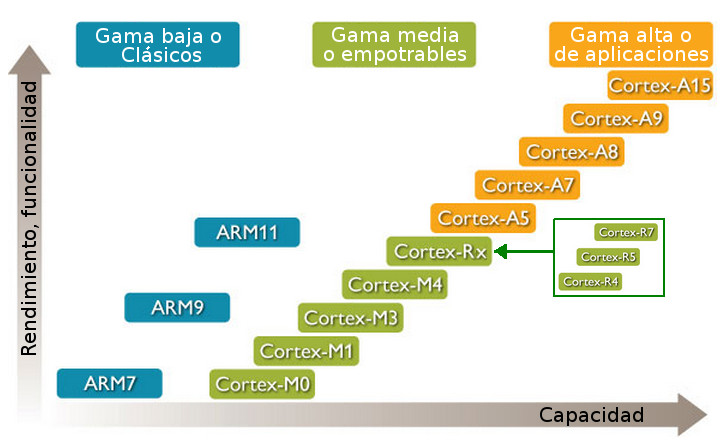
\includegraphics[width=13cm]{graphs/ArmRoadMap.jpg}
%  \caption{Clasificación de Familias ARM}
%  \label{fig:clasif_fami}
%\end{figure}

El chip en concreto que lleva la Raspberry Pi es el BCM2835, se trata de
un SoC (System on a Chip=Sistema en un sólo chip) que contiene además de
la CPU otros elementos como un núcleo GPU (hardware acelerado OpenGL
ES/OpenVG/Open EGL/OpenMAX y decodificación H.264 por hardware) y un
núcleo DSP (Digital signal processing=Procesamiento digital de señales)
que es un procesador más pequeño y simple que el principal, pero
especializado en el procesado y representación de señales analógicas.
La CPU en cuestión es la ARM1176JZF-S, un chip de la familia ARM11 que
usa la arquitectura ARMv6k. 

\begin{longtable}{| p{4.2cm} | p{2.5cm} | p{1cm} | p{6cm} |}
\hline
{\bf Familia} & {\bf Arquitectura} & {\bf Bits} & {\bf Ejemplos de dispositivos} \\ \hline
ARM1      & ARMv1       & 32/26 & Segundo procesador BBC Micro \\ \hline
ARM2, ARM3, Amber & ARMv2      & 32/26 & Acorn Archimedes \\ \hline
ARM6, ARM7 & ARMv3      & 32 & Apple Newton Serie 100 \\ \hline
ARM8, StrongARM & ARMv4       & 32 & Apple Newton serie 2x00 \\ \hline
ARM7TDMI,\newline ARM9TDMI & ARMv4T & 32 & Game Boy Advance \\ \hline
ARM7EJ, ARM9E,\newline ARM10E, XScale & ARMv5 & 32 & Samsung Omnia,\newline Blackberry 8700 \\ \hline
ARM11     & ARMv6 & 32 & iPhone 3G, Raspberry Pi \\ \hline
Cortex-M0/M0+/M1 & ARMv6-M & 32 & \\ \hline
Cortex-M3/M4 & ARMv7-M ARMv7E-M & 32 & Texas Instruments Stellaris \\ \hline
Cortex-R4/R5/R7 & ARMv7-R & 32 & Texas Instruments TMS570 \\ \hline
Cortex-A5/A7/A8/A9\newline A12/15/17, Apple A6 & ARMv7-A & 32 & Apple iPad \\ \hline
Cortex-A53/A57, X-Gene, Apple A7 & ARMv8-A & 64/32 & Apple iPhone 5S\\ \hline
\caption{Lista de familias y arquitecturas ARM}
\label{list_fam}
\end{longtable}

Las 
\textcolor{blue}{
  \href{http://infocenter.arm.com/help/index.jsp?topic=/com.arm.doc.ddi0301h/apbs02s02.html}
  {extensiones de la arquitectura ARMv6k}}
frente a la básica ARMv6 son mínimas
por lo que a efectos prácticos trabajaremos con la arquitectura ARMv6.

\subsubsection{Registros}
La arquitectura ARMv6 presenta un conjunto de 17 registros (16 principales
más uno de estado) de 32 bits cada uno.
\newline

\begin{figure}[h]
  \centering
    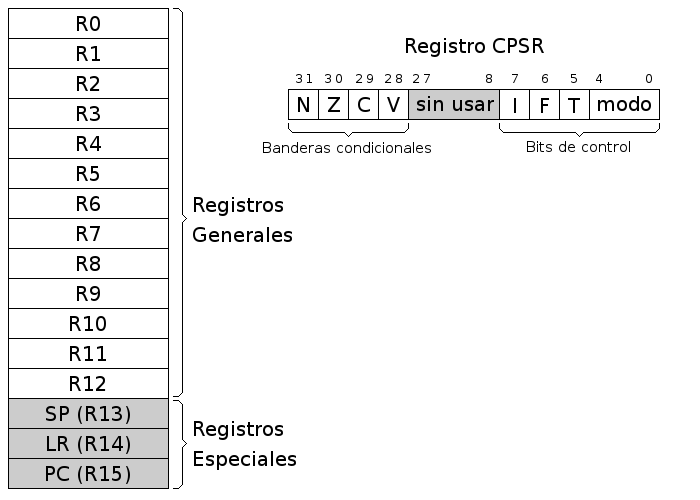
\includegraphics[width=14cm]{graphs/registros.png}
  \caption{Registros de la arquitectura ARM}
  \label{fig:reg_arm}
\end{figure}

\begin{descript}
  \item[Registros Generales.]
    Su función es el almacenamiento temporal de datos. Son los 13 registros
    que van R0 hasta R12.
  \item[Registros Especiales.]
    Son los últimos 3 registros principales: R13, R14 y R15. Como son de
    propósito especial, tienen nombres alternativos.

    \begin{itemize}
      \item{\textbf{SP}/R13. Stack Pointer ó Puntero de Pila. Sirve como puntero para almacenar
        variables locales y registros en llamadas a funciones.}
      \item{\textbf{LR}/R14. Link Register ó Registro de Enlace. Almacena la dirección de retorno
        cuando una instrucción BL ó BLX ejecuta una llamada a una rutina.}
      \item{\textbf{PC}/R15. Program Counter ó Contador de Programa. Es un registro que indica
        la posición donde está el procesador en su secuencia de instrucciones. Se
        incrementa de 4 en 4 cada vez que se ejecuta una instrucción, salvo que ésta
        provoque un salto.}
    \end{itemize}

  \item[Registro CPSR.]
        Almacena las banderas condicionales y los bits de control. Los bits de control
        definen la habilitación de interrupciones normales (I),
        interrupciones rápidas (F), modo Thumb \footnote{Es un modo simplificado donde las
        instrucciones son de 16 bits en lugar de 32 y se acceden a menos registros (hasta r7),
        con la ventaja de que el código ocupa menos espacio.} (T) y el modo de operación
        de la CPU. Existen hasta 8 modos de operación, pero por ahora desde nuestra aplicación
        sólo vamos a trabajar en uno de ellos, el {\it Modo Usuario}. Los demás son modos
        privilegiados usados exclusivamente por el sistema operativo.

        Desde el {\it Modo Usuario} sólo podemos acceder a las banderas condicionales, que
        contienen información sobre el estado de la última operación realizada por la ALU.
        A diferencia de otras arquitecturas en ARMv6 podemos elegir si queremos que una
        instrucción actualice o no las banderas condicionales, poniendo una ``s'' detrás
        del nemotécnico \footnote{Es la forma de nombrar las instrucciones desde
        ensamblador, normalmente derivadas de una abreviatura del verbo en inglés. Por
        ejemplo la instrucción {\it MOV} viene de ``move'' (mover) }. Existen 4 banderas
        y son las siguientes:

    \begin{itemize}
      \item{\textbf{N}. Se activa cuando el resultado es negativo.}
      \item{\textbf{Z}. Se activa cuando el resultado es cero o una comparación es cierta.}
      \item{\textbf{C}. Indica acarreo en las operaciones aritméticas.}
      \item{\textbf{V}. Desbordamiento aritmético.}
    \end{itemize}
\end{descript}


\subsubsection{Esquema de almacenamiento}

El procesador es {\it Bi-Endian}, quiere decir que es configurable entre {\it Big Endian}
y {\it Little Endian}. Aunque nuestro sistema operativo nos lo limita a {\it Little Endian}.

Por tanto la regla que sigue es ``el byte menos significativo ocupa la posición más baja''.
Cuando escribimos un dato en una posición de memoria, dependiendo de si es byte, half word
o word,... se ubica en memoria según el esquema de la figura \ref{fig:memo}. La dirección de un dato
es la de su byte menos significativo. La memoria siempre se referencia a nivel de byte, es
decir si decimos la posición N nos estamos refiriendo al byte N-ésimo, aunque se escriba
media palabra, una palabra,...

\begin{figure}[h]
  \centering
    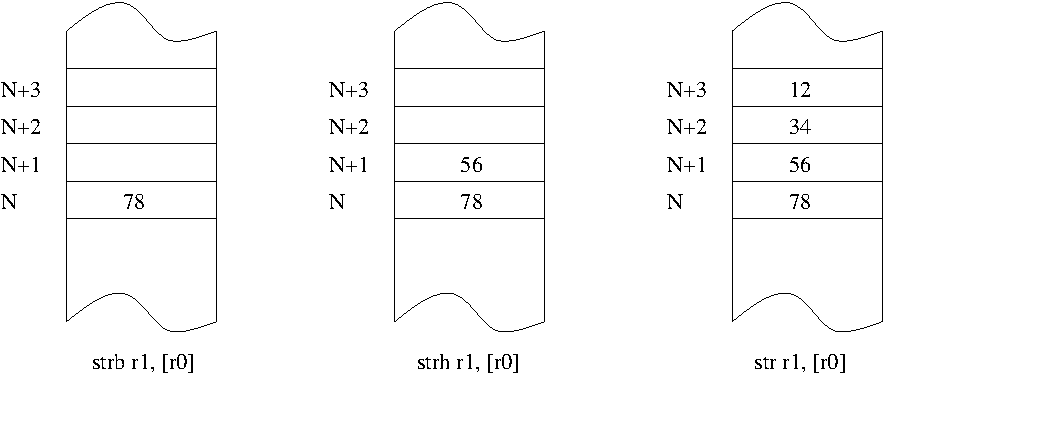
\includegraphics[width=13cm]{graphs/memo.pdf}
  \caption{Ubicación de datos en memoria}
  \label{fig:memo}
\end{figure}

\subsection{El lenguaje ensamblador}

El ensamblador es un lenguaje de bajo nivel que permite un control
directo de la CPU y todos los elementos asociados. Cada línea de un
programa ensamblador consta de una instrucción del procesador y la
posición que ocupan los datos de esa instrucción.

Desarrollar programas en lenguaje ensamblador es un proceso laborioso.
El procedimiento es similar al de cualquier lenguaje compilado.
Un conjunto de instrucciones y/o datos forman un módulo fuente.
Este módulo es la entrada del compilador, que chequea la sintaxis y lo
traduce a código máquina formando un módulo objeto.
Finalmente, un enlazador (montador ó {\it linker}) traduce todas las
referencias relativas a direcciones absolutas y termina generando el
ejecutable.

El ensamblador presenta una serie de ventajas e inconvenientes con
respecto a otros lenguajes de más alto nivel. Al ser un lenguaje de
bajo nivel, presenta como principal característica la flexibilidad y
la posibilidad de acceso directo a nivel de registro. En
contrapartida, programar en ensamblador es laborioso puesto que los
programas contienen un número elevado de líneas y la corrección y
depuración de éstos se hace difícil.

Generalmente, y dado que crear programas un poco extensos es
laborioso, el ensamblador se utiliza como apoyo a otros lenguajes
de alto nivel para 3 tipos de situaciones:
\begin{itemize}
     \item[-] Operaciones que se repitan un número elevado de veces.
     \item[-] Cuando se requiera una gran velocidad de proceso.
     \item[-] Para utilización y aprovechamiento de dispositivos y
     recursos del sistema.
\end{itemize}

\subsection{El entorno}

Los pasos habituales para hacer un programa (en cualquier lenguaje) son 
los siguientes:
lo primero es escribir el programa en el lenguaje fuente
mediante un editor de programas.
El resultado es un fichero en un lenguaje que puede entender el usuario,
pero no la máquina.
Para traducirlo a lenguaje máquina hay que utilizar un programa traductor.
Éste genera un fichero con la traducción de dicho programa, pero todavía
no es un programa ejecutable.
Un fichero ejecutable contiene el programa traducido más una serie de
códigos que debe tener todo programa que vaya a ser ejecutado en una
máquina determinada.
Entre estos códigos comunes se encuentran las librerías del lenguaje.
El encargado de unir el código del programa con el código de estas
librerías es un programa llamado montador ({\it linker}) que genera el
programa ejecutable (ver la figura \ref{fig:entorno})

\begin{figure}[h]
  \centering
    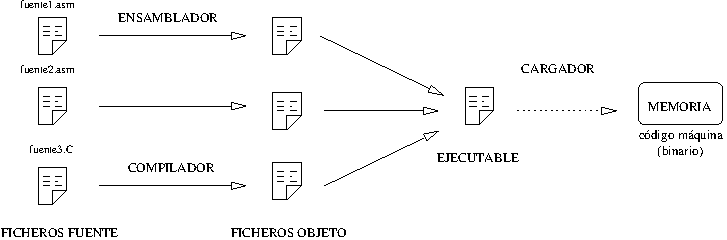
\includegraphics[width=13cm]{graphs/ensamblado.pdf}
  \caption{Entorno típico de programación}
  \label{fig:entorno}
\end{figure}

Durante el proceso de creación de un programa se suelen producir errores.
Hay dos tipos de errores: los sintácticos o detectables en tiempo de
traducción y los errores semánticos o detectables en tiempo de ejecución.
Los errores sintácticos son, por ejemplo, escribir mal una instrucción o
hacer una operación entre dos tipos de datos incompatibles.
Estos errores son detectados por el traductor y se deben solucionar para
poder generar un ejecutable.

Una vez que se tiene un programa sintácticamente correcto lo podemos
ejecutar, pero ésto no implica que el programa sea correcto. Todas las
instrucciones pueden ser correctas, pero se puede haber olvidado poner la
condición de salida de un bucle (y que no termine nunca) o que
sencillamente el programa no haga lo que queremos.

Estos errores sólo se pueden detectar en tiempo de ejecución.
Para poder eliminarlos se utiliza un depurador de programas ({\it debugger}).
El depurador nos permite ejecutar el programa instrucción a instrucción y
ver todos los valores que se van a calcular, de manera que podemos encontrar
los errores.

En el laboratorio utilizaremos el editor {\bf nano} para crear
y editar los módulos fuente de nuestros programas. El traductor
(que en el caso de traducir de un lenguaje ensamblador a lenguaje máquina
recibe el nombre de ensamblador), el {\it linker} y el {\it debugger} son
respectivamente GNU Assembler ({\bf as}), GNU Compiler Collection ({\bf gcc})
y GNU Debbuger ({\bf gdb}). Todas estas herramientas forman parte de la
GNU toolchain que viene instalada por defecto en la mayoría de las distribuciones
basadas en Linux, en concreto Raspbian. Para obtener más información sobre estos
comandos se puede recurrir a la ayuda del sistema con {\tt man as}, {\tt man gcc} y
{\tt man gdb}.

\subsection{Configuración del entorno para realizar las prácticas en casa}

Las instrucciones vienen detalladas en esta dirección:\newline
\textcolor{blue}{
  \href{http://elinux.org/RPi\_Easy\_SD\_Card\_Setup}
  {http://elinux.org/RPi\_Easy\_SD\_Card\_Setup}}

Vamos a hacer un resumen de cómo se haría en Windows. Para otros
sistemas operativos (Linux, Mac OS) seguir las instrucciones antes mencionadas.

\begin{enumerate}
  \item Descargamos la última versión de RASPBIAN en la siguiente url: \newline
\hspace{2.5cm}
\textcolor{blue}{
  \href{http://www.raspberrypi.org/downloads/}
  {http://www.raspberrypi.org/downloads/}}
  \item Extraemos del .zip el archivo de imagen, en nuestro caso se llama
        2014-01-07-wheezy-raspbian.img, aunque seguramente tu versión será más moderna.
  \item Insertamos una tarjeta SD en tu PC (slot SD o adaptador USB) y nos aseguramos de que
        funcione correctamente. Si no, la formateamos en FAT32.
  \item Nos bajamos e instalamos la utilidad Win32DiskImager. \newline
\hspace{2.5cm}
\textcolor{blue}{
  \href{http://sourceforge.net/projects/win32diskimager}
  {http://sourceforge.net/projects/win32diskimager}}
  \item Ejecutamos como Administrador la utilidad anterior.
  \item Dentro de la utilidad, seleccionamos el archivo de imagen anterior,
        2014-01-07-wheezy-raspbian.img
  \item Seleccionamos en Device la letra de unidad que nos apareció en el paso 3.
        Debemos asegurarnos de que la letra sea la correcta, de lo contrario
        podríamos destruir los datos de nuestro disco duro.
  \item Pulsamos el botón Write y esperamos a que se complete la escritura.
  \item Salimos de la utilidad y extraemos la tarjeta SD.
  \item Ya estamos listos para introducir la tarjeta SD en nuestra Raspberry Pi.
\end{enumerate}

De forma alternativa podemos ejecutar la imagen anterior en un emulador de
Raspberry Pi, y seguir gran parte de las prácticas con la comodidad de tu PC. Para
ello partimos del archivo de imagen obtenido en el apartado 2 de la lista anterior,
y seguimos los pasos según \cite{QEMU}. Los pasos son válidos para Windows y Linux,
aunque nosotros mostraremos sólo los de Windows.

\begin{enumerate}
  \item Descargamos el emulador QEMU desde aquí: \newline
\hspace{2.5cm}
\textcolor{blue}{
  \href{http://lassauge.free.fr/qemu/}
  {http://lassauge.free.fr/qemu/}}
  \item Descargamos el siguiente núcleo o kernel desde aquí: \newline
\hspace{2.5cm}
\textcolor{blue}{
  \href{http://xecdesign.com/downloads/linux-qemu/kernel-qemu}
  {http://xecdesign.com/downloads/linux-qemu/kernel-qemu}}
  \item Lanzamos la línea de comandos o ventana de MS-DOS. Esto se hace desde
{\tt Programas->Accesorios->Símbolo del sistema} o bien pulsando {\tt Windows+R} y escribiendo
``cmd''. Una vez lanzada escribimos lo siguiente:
\begin{lstlisting}
qemu-system-armw -kernel kernel-qemu -cpu arm1176
-m 256 -M versatilepb -no-reboot -serial stdio -append
"root=/dev/sda2 panic=1 rootfstype=ext4 rw init=/bin/bash"
-hda 2014-01-07-wheezy-raspbian.img
\end{lstlisting}
  \item Aparece el emulador en una nueva ventana tipo terminal. Ya estaríamos
dentro de la Raspberry emulada. Una vez se muestren los mensajes de arranque
aparece el siguiente texto:
\begin{lstlisting}
raspberrypi login:
\end{lstlisting}
  Nos está pidiendo el nombre de usuario. Nosotros escribimos {\tt pi}.
  \item Luego nos piden el password, que es {\tt raspberry}. En este caso y
por motivos de seguridad no se recibe respuesta visual mientras escribimos
la contraseña, ni siquiera aparecen asteriscos.
  \item Una vez identificados, lo primero que hacemos es editar el archivo
{\tt /etc/ld.so.preload} con el siguiente comando:
\begin{lstlisting}
nano /etc/ld.so.preload
\end{lstlisting}
  \item Dentro del editor ponemos un {\bf \#} al comienzo de la siguiente línea:
\begin{lstlisting}
#/usr/lib/arm-linux-gnueabihf/libcofi_rpi.so
\end{lstlisting}
  \item Presionamos {\tt Ctrl-X} y luego {\tt y}, Enter para guardar y salir.
  \item Escribimos {\tt sudo halt} para salir limpiamente del sistema emulado.
  \item Cerramos la ventana de QEMU y creamos el siguiente archivo {\tt lanzador.bat}.
\begin{lstlisting}
qemu-system-armw -kernel kernel-qemu -cpu arm1176
-m 256 -M versatilepb -no-reboot -serial stdio -append
"root=/dev/sda2 panic=1 rootfstype=ext4 rw"
-hda 2014-01-07-wheezy-raspbian.img
\end{lstlisting}
  \item Ejecutamos el archivo {\tt lanzador.bat} que acabamos de crear.
Ya hemos terminado. Todos los archivos que vayamos creando
se almacenan en la imagen como si se tratase de una SD real corriendo sobre una
Raspberry Pi real.
\end{enumerate}

\subsection{Aspecto de un programa en ensamblador}

En el listado \ref{lst:codigoPract1} se muestra el código de la primera
práctica que probaremos. En el código hay una serie de elementos que
aparecerán en todos los programas y que estudiaremos a continuación.

\begin{lstlisting}[caption={Código del programa intro1.s},label={lst:codigoPract1}]
.data

var1:   .word   3
var2:   .word   4
var3:   .word   0x1234

.text
.global main
 
main:   ldr     r1, puntero_var1    /* r1 <- &var1    */
        ldr     r1, [r1]            /* r1 <- *r1      */
        ldr     r2, puntero_var2    /* r2 <- &var2    */
        ldr     r2, [r2]            /* r2 <- *r2      */
        ldr     r3, puntero_var3    /* r3 <- &var3    */
        add     r0, r1, r2          /* r0 <- r1 + r2  */
        str     r0, [r3]            /* *r3 <- r0      */
        bx      lr

puntero_var1:   .word   var1
puntero_var2:   .word   var2
puntero_var3:   .word   var3
\end{lstlisting}

La principal característica de un módulo fuente en ensamblador es
que existe una clara separación entre las instrucciones y los
datos. La {\it estructura más general de un módulo fuente} es:

\begin{description}
     \item[* Sección de datos.] Viene identificada por la directiva {\it .data}.
En esta zona se definen todas las variables que utiliza el programa
con el objeto de reservar memoria para contener los valores asignados. Hay que
tener especial cuidado para que los datos estén alineados en palabras de 4 bytes,
sobre todo después de las cadenas. Alinear significa rellenar con ceros el final
de un dato para que el siguiente dato comience en una dirección múltiplo de 4 (con
los dos bits menos significativos a cero). Los datos son modificables.

     \item[* Sección de código.] Se indica con la directiva {\it .text}, y sólo
puede contener código o datos no modificables. Como todas las instrucciones son
de 32 bits no hay que tener especial cuidado en que estén alineadas. Si tratamos
de escribir en esta zona el ensamblador nos mostrará un mensaje de error.
\end{description}

De estas dos secciones la única que obligatoriamente debe existir es
la sección .text (o sección de código). En el ejemplo \ref{lst:codigoPract1}
comprobamos que están las dos.

Un módulo fuente, como el del ejemplo, está formado por instrucciones,
datos, símbolos y directivas. 
Las instrucciones son representaciones nemotécnicas del juego
de instrucciones del procesador. Un dato es una entidad que aporta un valor
numérico, que puede expresarse en distintas bases o incluso a través de una cadena.
Los símbolos son representaciones abstractas que el ensamblador maneja en tiempo
de ensamblado pero que en el código binario resultante tendrá un valor numérico
concreto. Hay tres tipos de símbolos: las etiquetas, las macros y las constantes simbólicas.
Por último tenemos las directivas, que sirven para indicarle ciertas cosas al
ensamblador, como delimitar secciones, insertar datos, crear macros, constantes
simbólicas, etc... Las instrucciones se aplican en tiempo de ejecución
mientras que las directivas se aplican en tiempo de ensamblado.

\subsubsection{Datos}

Los datos se pueden representar de distintas maneras. Para representar números tenemos
4 bases. La más habitual es en su forma decimal, la cual no lleva ningún delimitador
especial. Luego tenemos otra muy útil que es la representación hexadecimal, que
indicaremos con el prefijo {\it 0x}. Otra interesante es la binaria, que emplea el
prefijo {\it 0b} antes del número en binario. La cuarta y última base es la
octal, que usaremos en raras ocasiones y se especifica con el prefijo {\it 0}. Sí, un
cero a la izquierda de cualquier valor convierte en octal dicho número. Por ejemplo
015 equivale a 13 en decimal. Todas estas bases pueden ir con un signo menos delante,
codificando el valor negativo en complemento a dos. Para representar carácteres y cadenas
emplearemos las comillas simples y las comillas dobles respectivamente.

\subsubsection{Símbolos}

Como las etiquetas se pueden ubicar tanto en la sección de datos como en la de código,
la versatilidad que nos dan las mismas es enorme. En la zona de datos, las etiquetas pueden representar
variables, constantes y cadenas. En la zona de código podemos usar etiquetas de salto, funciones y
punteros a zona de datos.

Las macros y las constantes simbólicas son símbolos cuyo ámbito pertenece al preprocesador,
a diferencia de las etiquetas que pertenecen al del ensamblador. Se especifican con las
directivas .macro y .equ respectivamente y permiten que el código sea más legible y menos
repetitivo.

\subsubsection{Instrucciones}

Las instrucciones del {\bf as} (a partir de ahora usamos {\bf as} para referirnos al
ensamblador) responden al formato general:

\begin{lstlisting}
Etiqueta:  Nemotécnico  Operando/s  /* Comentario */
\end{lstlisting}

De estos campos, sólo el nemónico (nombre de la instrucción) es obligatorio. En
la sintaxis del {\bf as} cada instrucción ocupa una línea terminando preferiblemente
con el ASCII 10 (LF), aunque son aceptadas las 4 combinaciones: CR, LF, CR LF y LF CR.
Los campos se separan entre sí por al menos un carácter espacio (ASCII 32) o un tabulador
y no existe distinción entre mayúsculas y minúsculas.

\begin{lstlisting}
main:   ldr     r1, puntero_var1    /* r1 <- &var1    */
\end{lstlisting}

El Campo {\it etiqueta}, si aparece, debe estar formado por una
cadena alfanumérica. La cadena no debe comenzar con un dígito y no se puede
utilizar como cadena alguna palabra reservada del {\bf as} ni nombre
de registro del microprocesador. En el ejemplo, la etiqueta es
{\tt main:}.

El campo \textit{Nemotécnico} ({\tt ldr} en el ejemplo) es una forma
abreviada de nombrar la instrucción del procesador.
Está formado por caracteres alfabéticos (entre 1 y 11 caracteres).

El campo \textit{Operando/s} indica dónde se encuentran los datos.
Puede haber 0, 1 ó más operandos en una instrucción. Si hay más de uno
normalmente al primero se le denomina destino (salvo excepciones como {\tt str})
y a los demás fuentes, y deben ir separados por una coma.
Los operandos pueden ser registros, etiquetas, valores inmediatos o incluso
elementos más complejos como desplazadores/rotadores o indicadores de
pre/post-incrementos. En cualquiera de los casos el tamaño debe ser una
palabra (32 bits), salvo contadas excepciones como {\tt ldr} y {\tt str}
donde puede ser media palabra (16 bits) o un byte (8 bits).
En el ejemplo {\tt r1} es el operando destino, de tipo registro,
y {\tt puntero\_var1} es el operando fuente, una etiqueta. Tanto {\tt r1}
como {\tt puntero\_var1} hacen referencia a un valor de tamaño palabra (32 bits).

El campo \textit{Comentario} es opcional ({\tt r1 <- \&var1}, en el ejemplo)
y debe comenzar con la secuencia {\tt /*} y acabar con {\tt */} al igual
que los comentarios multilínea en C. No es obligatorio que estén a la
derecha de las instrucciones, aunque es lo habitual. También es común
verlos al comienzo de una función (ocupando varias líneas) para explicar
los parámetros y funcionalidad de la misma.

Cada instrucción del {\bf as} se refiere a una operación que puede
realizar el microprocesador. También hay pseudoinstrucciones que son
tratadas por el preprocesador como si fueran macros y codifican otras
instrucciones, como {\tt lsl rn, \#x} que codifica {\tt mov rn, rn, lsl \#x},
o bien {\tt push/pop} que se traducen instrucciones {\tt stm/ldm} más complejas
y difíciles de recordar para el programador. Podemos agrupar el conjunto de
instrucciones del {\bf as}, según el tipo de función que realice el
microprocesador, en las siguientes categorías:

\begin{itemize}

       \item \textit{Instrucciones de transferencia de datos}
Mueven información entre registros y posiciones de memoria. En la
arquitectura ARMv6 no existen puertos ya que la E/S está mapeada
en memoria. Pertenecen a este grupo las siguientes instrucciones:
\textbf{mov, ldr, str, ldm, stm, push, pop}.

       \item \textit{Instrucciones aritméticas.}  Realizan operaciones
aritméticas sobre números binarios o BCD.  Son instrucciones de este
grupo \textbf{add, cmp, adc, sbc, mul}.

     \item \textit{Instrucciones de manejo de bits.}  Realizan
operaciones de desplazamiento, rotación y lógicas sobre registros o
posiciones de memoria. Están en este grupo las instrucciones:\textbf{
and, tst, eor, orr, LSL, LSR, ASR, ROR, RRX}.

     \item \textit{Instrucciones de transferencia de control.}  Se
utilizan para controlar el flujo de ejecución de las instrucciones
del programa. Tales como \textbf{b, bl, bx, blx} y sus variantes
condicionales.

\end{itemize}

En esta sesión práctica se explorarán algunas de estas instrucciones.
Para buscar información sobre cualquiera de ellas durante las prácticas,
recuerda que puedes utilizar el manual técnico del ARM1176JZF-S \cite{ATRM}.

\subsubsection{Directivas}

Las directivas son expresiones que aparecen en el módulo fuente e
indican al compilador que realice determinadas tareas en el proceso
de compilación. Son fácilmente distinguibles de las instrucciones
porque siempre comienzan con un punto. El uso de directivas es
aplicable sólo al entorno del compilador, por tanto varían de un
compilador a otro y para diferentes versiones de un mismo compilador.
Las directivas más frecuentes en el {\bf as} son:

\begin{itemize}
        \item \textit{Directivas de asignación:} Se utilizan para dar
valores a las constantes o reservar posiciones de memoria para las
variables (con un posible valor inicial).  \textbf{.byte, .hword, .word,
.ascii, .asciz, .zero y .space}
son directivas que indican al compilador que reserve memoria para
las variables del tipo indicado. Por ejemplo:

\begin{lstlisting}
a1:   .byte  1       /* tipo byte, inicializada a 1 */
var2: .byte  'A'     /* tipo byte, al caracter 'A'  */
var3: .hword 25000   /* tipo hword (16 bits) a 25000*/
var4: .word 0x12345678 /* tipo word de 32 bits      */
b1:   .ascii "hola"  /* define cadena normal        */
b2:   .asciz "ciao"  /* define cadena acabada en NUL*/
dat1: .zero  300     /* 300 bytes de valor cero     */
dat2: .space 200, 4  /* 200 bytes de valor 4        */
\end{lstlisting}

La directiva \textbf{.equ} (ó \textbf{.set}) es utilizada para asignar un
valor a una constante simbólica:

\begin{lstlisting}
.equ N, -3     /* en adelante N se sustituye por -3 */
\end{lstlisting}

\item \textit{Directivas de control:}
        \textbf{.text y .data} sirven para delimitar las distintas secciones
        de nuestro módulo.
        \textbf{.align {alineamiento}} es para alinear el siguiente dato,
        rellenando con ceros, de tal forma que comience en una dirección
        múltiplos del número que especifiquemos en {\it alineamiento},
        normalmente potencia de 2. Si no especificamos {\it alineamiento}
        por defecto toma el valor de 4 (alineamiento a palabra):

\begin{lstlisting}
a1: .byte 25   /* definimos un byte con el valor 25 */
    .align     /* directiva que rellena con 3 bytes */
a2: .word 4    /* variable alineada a tamaño palabra*/
\end{lstlisting}

        \textbf{.include} para incluir un archivo fuente dentro del actual.
        \textbf{.global} hace visible al enlazador el símbolo que hemos
        definido con la etiqueta del mismo nombre.

     \item \textit{Directivas de operando:} Se aplican a los datos en
        tiempo de compilación. En general, incluyen las operaciones lógicas
        {\tt \&}, {\tt |}, {\tt $\sim$}, aritméticas {\tt +}, {\tt -},
        {\tt *}, {\tt /}, {\tt \%} y de desplazamiento
        {\tt $<$}, {\tt $>$}, {\tt $<<$}, {\tt $>>$}:

\begin{lstlisting}
.equ pies, 9     /* definimos a 9 la constante pies */
.equ yardas, pies/3     /* calculamos las yardas= 3 */
.equ pulgadas, pies*12  /* calculamos pulgadas= 108 */
\end{lstlisting}

     \item \textit{Directivas de Macros:} Una {\it .macro} es un
conjunto de sentencias en ensamblador (directivas e instrucciones) que
pueden aparecer varias veces repetidas en un programa con algunas
modificaciones (opcionales). Por ejemplo, supongamos que a lo largo de
un programa realizamos varias veces la operación $n^{2}+1$ donde n y el
resultado son registros. Para acortar el código a escribir
podríamos usar una macro como la siguiente:

\begin{lstlisting}
    .macro CuadM1 input, aux, output
        mul     aux, input, input
        add     output, aux, #1
    .endm    
\end{lstlisting}

Esta macro se llama {\it CuadM1} y tiene tres parámetros (input, aux y output).
Si posteriormente usamos la macro de la siguiente forma:

\begin{lstlisting}
        CuadM1  r1, r8, r0
\end{lstlisting}

\noindent el ensamblador se encargará de expandir la macro, es decir, en lugar de
la macro coloca:

\begin{lstlisting}
        mul     r8, r1, r1
        add     r0, r8, #1
\end{lstlisting}

No hay que confundir las macros con los procedimientos. Por un lado,
el código de un procedimiento es único, todas las llamadas usan el
mismo, mientras que el de una macro aparece (se expande) cada vez que
se referencia, por lo que ocuparán más memoria. Las macros serán
más rápidas en su ejecución, pues es secuencial, frente a
los procedimientos, ya que implican un salto cuando aparece la llamada
y un retorno cuando se termina. La decisión de usar una macro o un
procedimiento dependerá de cada situación en concreto, aunque las
macros son muy flexibles (ofrecen muchísimas más posibilidades de las
comentadas aquí). Esta posibilidad será explotada en sesiones más avanzadas.

\end{itemize}

\subsection{Ensamblar y {\it linkar} un programa}

La traducción o ensamblado de un módulo fuente ({\bf nombreprograma.s})
se realiza con el programa Gnu Assembler, con el siguiente comando:

\begin{lstlisting}
        as -o nombreprograma.o nombreprograma.s
\end{lstlisting}

NOTA: tanto el comando {\bf as} como el nombre del programa son sensibles
a las mayúsculas. Por tanto el comando debe ir en minúsculas y el nombre
como queramos, pero recomendamos minúsculas también.
Las opción {\bf -o nombreprograma.o} puede ir después de {\bf nombreprograma.s}.

El {\bf as} genera un fichero nombreprograma.o.

Para montar ({\it linkar}) hay que hacer:

\begin{lstlisting}
        gcc -o nombreprograma nombreprograma.o
\end{lstlisting}

NOTA: Nuevamente, tanto {\bf gcc} como el nombre del programa deben estar
en minúsculas. Este comando es muy parecido al anterior, podemos poner si
queremos {\bf -o nombreprograma} detrás de {\bf nombreprograma.o}. La única
diferencia es que el archivo no tiene extensión, que por otro lado es una
práctica muy recomendable para ejecutables en Linux.

Una vez hecho ésto, ya tenemos un fichero ejecutable (nombreprograma) que
podemos ejecutar o depurar con el {\bf gdb}.

\section{Enunciados de la práctica}

\subsection{Cómo empezar}

Recuerda que en laboratorio las raspberries no tienen
monitor ni teclado, la única conexión con el mundo real
es el puerto Ethernet. En el apéndice \ref{chp:SerieBoot} se
explica otro mecanismo para conectar.

Así que antes de nada averigua cuál es la dirección IP de la Raspberry
Pi dentro de la red local. Por defecto el usuario es {\tt pi} y la
contraseña {\tt raspberry}. Suponiendo que la dirección IP asignada es
{\tt 192.168.1.42}, utilizaremos ssh:

\begin{lstlisting}[language=bash]
        ssh pi@192.168.1.42
\end{lstlisting}

Y luego introduce la contraseña. Ya conectado a la Raspberry Pi desde un PC
a través de ssh. Todos los alumnos se conectarán con el mismo nombre de usuario,
por lo que hay que dejar limpio el directorio de trabajo antes de terminar
la sesión.

También es buena idea conectarte por ssh a la Raspberry que tengas en casa
como acabamos de explicar, así te ahorras el tener que disponer de teclado
y monitor extra. Desde Windows puedes bajarte putty.exe 
en \newline
\textcolor{blue}{
  \href{http://www.chiark.greenend.org.uk/~sgtatham/putty/download.html}
  {http://www.chiark.greenend.org.uk/~sgtatham/putty/download.html}}
(no requiere instalación) y crear un acceso directo en el escritorio con
el siguiente destino, cambiando {\bf ruta} y {\bf 192.168.1.42} por lo que
corresponda.

\begin{lstlisting}
C:\ruta\putty.exe 192.168.1.42 -l pi -pw raspberry
\end{lstlisting}

Comenzaremos con el programa que hemos visto en el listado
\ref{lst:codigoPract1}, y que se encuentra en el fichero {\tt intro1.s}.
Edítalo con el programa {\bf nano} para verlo (y practicar un poco):

\begin{lstlisting}
        nano intro1.s
\end{lstlisting}

Dentro del editor tenemos una pequeña guía de comandos en la parte
inferior. También podemos acceder a una ayuda más detallada pulsando {\bf F1}
dentro del editor. Estos son los atajos de teclado más comunes:

\begin{longtable}{| p{1.3cm} | p{12cm} |}
\hline
{\bf Atajo} & {\bf Función} \\ \hline
Ctrl-x & Salir de nano, se pide confirmación con Y/N \\ \hline
Ctrl-o & Salvar cambios \\ \hline
Ctrl-c & Muestra panel con información sobre número de línea \\ \hline
Alt-g  & Saltar a un número de línea en concreto \\ \hline
Alt-a ó\newline
Ctrl-6 & Seleccionar texto, mover cursores para definir región  \\ \hline
Alt-\^ & Copiar selección \\ \hline
Ctrl-k & Cortar selección \\ \hline
Ctrl-u & Pegar selección \\ \hline
Ctrl-w & Buscar texto \\ \hline
Alt-w  & Repetir última búsqueda \\ \hline
Alt-r  & Buscar y reemplazar \\ \hline
\caption{Lista de atajos de teclado para editor nano}
\label{list_nano}
\end{longtable}

Una vez que estéis familiarizados con el {\bf nano} podemos pasar al
traductor:

\begin{lstlisting}
        as -o intro1.o intro1.s
\end{lstlisting}

Observa que cuando se traduce, aparece una lista de errores, o bien, una
indicación de que el programa se ha traducido correctamente.
No se puede pasar a la etapa de montaje hasta que no se han solucionado
los errores de sintaxis.

\begin{lstlisting}
        gcc -o intro1 intro1.o
\end{lstlisting}

De la misma forma, el montador nos informa de si todo el proceso ha sido
correcto.

Una vez que hemos terminado con éxito este proceso podemos pasar el programa al
{\bf gdb} (GNU Debugger).

\begin{lstlisting}
        gdb intro1
\end{lstlisting}

El {\bf gdb} ofrece muchas posibilidades, sólo explicaremos las que vamos
a utilizar. Nada más ejecutar el comando anterior, el {\bf gdb} se encuentra
en modo interactivo:

\begin{lstlisting}[language=bash]
pi@raspberrypi ~ $ gdb intro1
GNU gdb (GDB) 7.4.1-debian
Copyright (C) 2012 Free Software Foundation, Inc.
License GPLv3+: GNU GPL version 3 or later 
This is free software: you are free to change and redis...
There is NO WARRANTY, to the extent permitted by law.  ...
and "show warranty" for details.
This GDB was configured as "arm-linux-gnueabihf".
For bug reporting instructions, please see:
...
Reading symbols from /home/pi/intro1...(no debugging sy...
(gdb)
\end{lstlisting}

Podemos escribir {\bf help} para acceder a la ayuda integrada, o bien
irnos a la página web de documentación del {\bf gdb} \cite{DGDB}.
El primer comando a aprender es:

\begin{lstlisting}
(gdb) quit
\end{lstlisting}

Lanzamos de nuevo el depurador {\bf gdb intro1}. En este momento no hay
nada ejecutándose. Un primer paso es decirle al depurador que queremos
lanzar el programa, esto es, cargarlo en memoria y apuntar a la primera
instrucción del mismo:

\begin{lstlisting}
(gdb) start
Temporary breakpoint 1 at 0x8390
Starting program: /home/pi/intro1
 
Temporary breakpoint 1, 0x00008390 in main ()
\end{lstlisting}

Perfecto, nos hemos saltado todos los pasos de inicialización de la
librería C y estamos a punto de ejecutar la primera instrucción de
nuestra función main. Veamos qué hay allí:

\begin{lstlisting}
(gdb) disassemble
Dump of assembler code for function main:
=> 0x00008390: ldr r1, [pc, #24];  0x83b0 <puntero_var1>
   0x00008394: ldr r1, [r1]
   0x00008398: ldr r2, [pc, #20];  0x83b4 <puntero_var2>
   0x0000839c: ldr r2, [r2]
   0x000083a0: ldr r3, [pc, #16];  0x83b8 <puntero_var3>
   0x000083a4: add r0, r1, r2
   0x000083a8: str r0, [r3]
   0x000083ac: bx  lr
End of assembler dump.
\end{lstlisting}

Vemos que las instrucciones que hacían referencia a {\bf puntero\_varX}
han cambiado. De momento lo ignoramos, ya lo explicaremos más adelante.
Observen que hay una especie de flecha {\bf $=>$} apuntando a la
instrucción que está apunto de ejecutarse (no lo ha hecho aún).
Antes de ejecutarla, veamos los valores de algunos registros:

\newpage
\begin{lstlisting}
(gdb) info registers r0 r1 r2 r3
r0             0x1              1
r1             0xbefffe04       3204447748
r2             0xbefffe0c       3204447756
r3             0x8390           33680
\end{lstlisting}

Podemos modificar el valor de los registros por medio de la orden
{\bf print}, teniendo en cuenta los efectos adversos que esto podría
ocasionar, ya que estamos alterando el funcionamiento de nuestro
programa. En este caso no pasa nada, puesto que aún no hemos ejecutado
ninguna instrucción.

\begin{lstlisting}
(gdb) print $r0 = 2
$1 = 2
(gdb) info registers r0 r1 r2 r3
r0             0x2              2
r1             0xbefffe04       3204447748
r2             0xbefffe0c       3204447756
r3             0x8390           33680
\end{lstlisting}

{\bf gdb} muestra \$1, que es el identificador asignado al resultado. Podemos
usar dicho identificador en nuevas expresiones y así ahorramos tiempo al teclear.
En este ejemplo no es muy útil, pero lo será si la expresión es más compleja.

\begin{lstlisting}
(gdb) print $1
$2 = 2
\end{lstlisting}

Ahora podemos usar \$2, y así sucesivamente. Bueno, ya es hora de ejecutar la primera
instrucción.

\begin{lstlisting}
(gdb) stepi
0x00008394 in main ()
\end{lstlisting}

Veamos qué ha pasado desensamblando de nuevo.

\begin{lstlisting}
(gdb) disassemble
Dump of assembler code for function main:
   0x00008390: ldr r1, [pc, #24];  0x83b0 <puntero_var1>
=> 0x00008394: ldr r1, [r1]
   0x00008398: ldr r2, [pc, #20];  0x83b4 <puntero_var2>
   0x0000839c: ldr r2, [r2]
   0x000083a0: ldr r3, [pc, #16];  0x83b8 <puntero_var3>
   0x000083a4: add r0, r1, r2
   0x000083a8: str r0, [r3]
   0x000083ac: bx  lr
End of assembler dump.
\end{lstlisting}

Observamos que la flecha {\bf $=>$} ha cambiado de posición, apuntando ahora
a la segunda instrucción. Veamos qué le ha pasado a {\bf r1}.

\begin{lstlisting}
(gdb) info register r1
r1             0x10558  66904
\end{lstlisting}

Bien, ha cambiado. De hecho esta es la dirección de {\bf puntero\_var1}.
Comprobémoslo usando su nombre simbólico con la sintaxis de C.

\begin{lstlisting}
(gdb) print &var1
$3 = ( *) 0x10558 <puntero_var1>
\end{lstlisting}

Genial. Ahora veamos el contenido de dicha variable.

\begin{lstlisting}
(gdb) print var1
$4 = 3
\end{lstlisting}

Perfecto, es lo que esperábamos. Veamos el siguiente paso.

\begin{lstlisting}
(gdb) stepi
0x00008398 in main ()
(gdb) disas
Dump of assembler code for function main:
   0x00008390: ldr r1, [pc, #24];  0x83b0 <puntero_var1>
   0x00008394: ldr r1, [r1]
=> 0x00008398: ldr r2, [pc, #20];  0x83b4 <puntero_var2>
   0x0000839c: ldr r2, [r2]
   0x000083a0: ldr r3, [pc, #16];  0x83b8 <puntero_var3>
   0x000083a4: add r0, r1, r2
   0x000083a8: str r0, [r3]
   0x000083ac: bx  lr
End of assembler dump.
\end{lstlisting}

Puedes emplear {\bf disas} (pero no {\bf disa}) como comando
abreviado. En realidad todos los comandos pueden abreviarse, sólo
que no lo hemos hecho para os resulte más fácil su memorización.
A partir de ahora pondré versiones abreviadas de comandos que ya
hayamos mostrado.

\begin{lstlisting}
(gdb) i r r1
r1             0x3  3
\end{lstlisting}

Vamos bien. Ahora ejecutamos hasta la instrucción {\bf str}, que
serían exactamente 4 pasos.

\begin{lstlisting}
(gdb) si 4
0x000083a8 in main ()
(gdb) disas
Dump of assembler code for function main:
   0x00008390: ldr r1, [pc, #24];  0x83b0 <puntero_var1>
   0x00008394: ldr r1, [r1]
   0x00008398: ldr r2, [pc, #20];  0x83b4 <puntero_var2>
   0x0000839c: ldr r2, [r2]
   0x000083a0: ldr r3, [pc, #16];  0x83b8 <puntero_var3>
   0x000083a4: add r0, r1, r2
=> 0x000083a8: str r0, [r3]
   0x000083ac: bx  lr
End of assembler dump.
\end{lstlisting}

Comprobamos ahora que la intrucción {\bf str} funciona correctamente,
inspeccionando la variable {\bf var3} antes y después.

\begin{lstlisting}
(gdb) p var3
$5 = 4660
(gdb) si
0x000083ac in main ()
(gdb) p var3
$6 = 7
\end{lstlisting}

Ahora ejecutemos hasta el final.

\begin{lstlisting}
(gdb) continue
Continuing.
[Inferior 1 (process 2477) exited with code 07]
\end{lstlisting}

El depurador nos indica que el código de salida es 07. Este código
se lo indicamos en el registro {\bf r0} justo antes de salir del {\bf main}.
Nos salimos del depurador y comprobamos que ejecutando el programa
directamente, aunque éste no muestre ninguna salida por pantalla, podemos
verificar su código de salida de la siguiente forma:

\begin{lstlisting}[language=bash]
pi@raspberrypi ~ $ ./intro1 ; echo $?
7
pi@raspberrypi ~ $
\end{lstlisting}

Ahora que ya tenemos una idea de las posibilidades del {\bf gdb}
vamos a repasar unos cuantos conceptos con la ayuda de este programa.

\subsection{Enteros y naturales}

Recordemos que cuando se representa cualquier dato en memoria, éste tiene un
valor explícito (el que tiene como dato guardado en binario) y un
valor implícito (el que tiene interpretado como un tipo de dato
determinado o como una instrucción). En este apartado queremos que veais la
diferencia entre el valor explícito y el valor implícito interpretado como
un natural y como un entero.

\subsubsection{Ejercicio 1.1}
Suponemos dos variables de longitud un byte {\tt var1}
y {\tt var2} con los valores binarios ($00110010_b$) y ($11000000_b$),
respectivamente. Completa las casillas en blanco.

\begin{center}
\small
\colorbox[gray]{0.9}{
%\arrayrulecolor{black}
\tabcolsep = 1mm
\begin{tabular}{ccccc}
& Valor explícito & Valor explícito & Valor implícito & Valor implícito \\
 & (binario) & (hexadecimal) & (como un natural & (como un entero \\
& & & en decimal) & en decimal) \\
var1 &
\colorbox[gray]{1}{\rule{0cm}{0.46cm}\rule{0.2cm}{0cm}00110010\rule{0.2cm}{0cm}} &
\colorbox[gray]{1}{\rule{0cm}{0.46cm}\rule{2.6cm}{0cm}} &
\colorbox[gray]{1}{\rule{0cm}{0.46cm}\rule{2.6cm}{0cm}} &
\colorbox[gray]{1}{\rule{0cm}{0.46cm}\rule{2.6cm}{0cm}} \\[1mm]
var2 &
\colorbox[gray]{1}{\rule{0cm}{0.46cm}\rule{0.2cm}{0cm}11000000\rule{0.2cm}{0cm}} &
\colorbox[gray]{1}{\rule{0cm}{0.46cm}\rule{2.6cm}{0cm}} &
\colorbox[gray]{1}{\rule{0cm}{0.46cm}\rule{2.6cm}{0cm}} &
\colorbox[gray]{1}{\rule{0cm}{0.46cm}\rule{2.6cm}{0cm}} \\
\end{tabular}
\vspace{0.5ex}
}
\end{center}

Observa que los valores son bien diferentes según la interpretación (valor
implícito) que se les dé.

\subsubsection{Ejercicio 1.2}
Calcula ahora la suma de los dos números y responde en las casillas en blanco.

\begin{center}
\small
\colorbox[gray]{0.9}{
\tabcolsep = 1mm
\begin{tabular}{cccc}
Valor explícito & Valor explícito & Valor implícito & Valor implícito \\
(binario) & (hexadecimal) & (como un natural & (como un entero \\
& & en decimal) & en decimal) \\
\colorbox[gray]{1}{
\begin{minipage}[b]{2cm}
\begin{flushright}
00110010\\
+11000000\\[-3mm]
\hrulefill
\end{flushright}
\vspace{0.4cm}
\end{minipage}
} &
= \colorbox[gray]{1}{\rule{0cm}{0.46cm}\rule{2cm}{0cm}} &
= \colorbox[gray]{1}{\rule{0cm}{0.46cm}\rule{2cm}{0cm}} &
= \colorbox[gray]{1}{\rule{0cm}{0.46cm}\rule{2cm}{0cm}} \\
\\
\multicolumn{2}{l}{
¿Cuál es el valor final de los flags?} &
\multicolumn{2}{l}{
\colorbox[gray]{1}{\rule{0cm}{0.46cm}N=\rule{0.7cm}{0cm}Z=\rule{0.7cm}{0cm}C=\rule{0.7cm}{0cm}V=\rule{0.7cm}{0cm}}
}\\[1mm]
\multicolumn{3}{l}{
¿Es el resultado final correcto interpretado como un natural?} &
\multicolumn{1}{l}{
\colorbox[gray]{1}{\rule{1cm}{0cm}\rule{0cm}{0.46cm}}} \\[1mm]
\multicolumn{3}{l}{
¿Es el resultado final correcto interpretado como un entero?} &
\multicolumn{1}{l}{
\colorbox[gray]{1}{\rule{1cm}{0cm}\rule{0cm}{0.46cm}}} \\
\end{tabular}
}
\end{center}

Ahora es el momento de comprobar si hemos contestado correctamente.
El código de esta parte se encuentra en el fichero {\tt intro2.s}
(listado \ref{lst:codigoPract2}).

\begin{lstlisting}[caption={Código del programa intro2.s},label={lst:codigoPract2}]
.data

var1:   .byte   0b00110010
        .align
var2:   .byte   0b11000000
        .align

.text
.global main
 
main:   ldr     r1, =var1     /* r1 <- &var1    */
        ldrsb   r1, [r1]      /* r1 <- *r1      */
        ldr     r2, =var2     /* r2 <- &var2    */
        ldrsb   r2, [r2]      /* r2 <- *r2      */
        add     r0, r1, r2    /* r0 <- r1 + r2  */
        bx      lr
\end{lstlisting}

Si os fijáis hemos hecho algunos cambios con respecto a {\tt intro1.s}. Las
variables son de tipo byte en lugar de word, lo que nos obliga a
alinear con {\bf .align} después de cada una. Las cargamos con la
instrucción {\bf ldrsb}, indicando que lo que cargamos es un byte {\bf b}
al que le extendemos su signo {\bf s}. Hemos eliminado la variable {\bf var3},
al fin y al cabo vamos a obtener el resultado en el registro {\bf r0}.
Por último hemos simplificado la carga de la dirección de la variables
con {\bf ldr r1, =var1}, de esta forma el ensamblador se encarga de declarar los
punteros automáticamente.

Ensámblalo, móntalo y síguelo con el {\bf gdb} tal y como se ha explicado en
la primera parte de la práctica. Ejecuta sólo las 5 primeras instrucciones.
Analiza el resultado del registro r0 y responde al siguiente ejercicio.

\subsubsection{Ejercicio 1.3}

\begin{center}
\small
\colorbox[gray]{0.9}{
\tabcolsep = 1mm
\begin{tabular}{rccc}
\multicolumn{3}{l}{Si interpretamos el resultado como byte}\\
\multicolumn{2}{c}{binario} & hexa \\
\multicolumn{2}{c}{\colorbox[gray]{1}{\rule{6cm}{0cm}\rule{0cm}{0.46cm}}}
& \colorbox[gray]{1}{\rule{2cm}{0cm}\rule{0cm}{0.46cm}} \\
\multicolumn{3}{l}{}\\
\multicolumn{3}{l}{Si interpretamos el resultado como palabra (32 bits)}\\
\multicolumn{2}{c}{binario} & hexa \\
\multicolumn{2}{c}{\colorbox[gray]{1}{\rule{6cm}{0cm}\rule{0cm}{0.46cm}}}
& \colorbox[gray]{1}{\rule{2cm}{0cm}\rule{0cm}{0.46cm}} \\
\multicolumn{3}{l}{}\\
\multicolumn{3}{l}{Ídem, pero si no hubiésemos extendido los signos}\\
\multicolumn{3}{l}{(ldrb en lugar de ldrsb)}\\
\multicolumn{2}{c}{binario} & hexa \\
\multicolumn{2}{c}{\colorbox[gray]{1}{\rule{6cm}{0cm}\rule{0cm}{0.46cm}}}
& \colorbox[gray]{1}{\rule{2cm}{0cm}\rule{0cm}{0.46cm}} \\
\end{tabular}
}
\end{center}

\subsubsection{Ejercicio 1.4}

Repite el ejercicio anterior, pero ahora comprobando el resultado de los
flags con lo que habías calculado en el Ejercicio 1.2. ¿Qué ocurre?

Si observáis, el registro cpsr no cambia, es el mismo antes y después de
ejecutar la instrucción {\bf add}.

\begin{lstlisting}
(gdb) i r cpsr
cpsr         0x60000010    1610612752
\end{lstlisting}

Por cierto, desde {\bf gdb} no hay una forma sencilla de obtener los flags
por separado. Por suerte son fáciles de interpretar a partir del valor
hexadecimal de {\bf cpsr}. Convertimos a binario el nibble (dígito hexadecimal)
más significativo de cpsr, en este caso 6 -> 0110. Hacemos corresponder 0110
con la secuencia {\bf NZCV} (debemos aprenderla de memoria),
con lo cual tendríamos N=0, Z=1, C=1 y V=0.

La razón por la que no se actualizan los flags es que el ensamblador del ARM no
lo hace a menos que se lo indiquemos con una {\bf s} detrás de la instrucción.
Cambiemos la línea 15 del archivo {\tt intro2.s} por ésta.

\begin{lstlisting}
        adds    r0, r1, r2    /* r0 <- r1 + r2  */
\end{lstlisting}

Y repetimos todos los pasos: ensamblado, enlazado y depuración. Ahora sí, comprueba
que los flags se corresponden con los valores calculados.

\subsection{Instrucciones lógicas}


\subsubsection{Ejercicio 1.5}
Supón que tienes dos variables de tamaño 1 byte, {\tt var1} y {\tt var2}, con los valores
$11110000_b$ y $10101010_b$. Calcula el resultado de hacer una operación
AND y una operación OR entre las dos variables.

\begin{center}
\small
\colorbox[gray]{0.9}{
\tabcolsep = 1mm
\begin{tabular}{cccccc}
         & Valor     & & Valor         & Valor     & \\
Variable & (binario) & & (hexadecimal) & (binario) & \\
var1 &
\colorbox[gray]{1}{\rule{0.3cm}{0cm}\rule{0cm}{0.46cm}11110000\rule{0.3cm}{0cm}}
& &
\colorbox[gray]{1}{\rule{2cm}{0cm}\rule{0cm}{0.46cm}} &
\colorbox[gray]{1}{\rule{0.3cm}{0cm}\rule{0cm}{0.46cm}11110000\rule{0.3cm}{0cm}}
& \\[1mm]
var2 &
\colorbox[gray]{1}{\rule{0.3cm}{0cm}\rule{0cm}{0.46cm}10101010\rule{0.3cm}{0cm}}
& &
\colorbox[gray]{1}{\rule{2cm}{0cm}\rule{0cm}{0.46cm}} &
\colorbox[gray]{1}{\rule{0.3cm}{0cm}\rule{0cm}{0.46cm}10101010\rule{0.3cm}{0cm}}
& \\[1mm]
\cline{2-3}\cline{5-6}\\[-3mm]
\multicolumn{1}{r}{var1 AND var2} &
\colorbox[gray]{1}{\rule{2cm}{0cm}\rule{0cm}{0.46cm}} &
\colorbox[gray]{1}{\rule{1cm}{0cm}\rule{0cm}{0.46cm}} &
\multicolumn{1}{r}{var1 OR var2} &
\colorbox[gray]{1}{\rule{2cm}{0cm}\rule{0cm}{0.46cm}} &
\colorbox[gray]{1}{\rule{1cm}{0cm}\rule{0cm}{0.46cm}} \\
& binario & hexa & & binario & hexa \\
\end{tabular}
}
\end{center}

Para comprobar el resultado tenemos el programa {\tt intro3.s}.

\begin{lstlisting}[caption={Código del programa intro3.s},label={lst:codigoPract3}]
.text
.global main
 
main:   mov     r2, #0b11110000   /* r2 <- 11110000   */
        mov     r3, #0b10101010   /* r3 <- 10101010   */
        and     r0, r2, r3        /* r0 <- r2 AND r3  */
        orr     r1, r2, r3        /* r1 <- r2 OR  r3  */
        mvn     r4, r0            /* r4 <- NOT r0     */
        mov     r0, #0x80000000
        tst     r0, #0x80000000
        tst     r0, #0x40000000
        bx      lr
\end{lstlisting}

Ejecuta las 4 primeras instrucciones y comprueba tus respuestas.

\subsubsection{Ejercicio 1.6}
El resultado de la instrucción {\tt and} está en r0. ¿Cuál será el resultado
de hacer un complemento a uno del mismo?

\begin{center}
\small
\colorbox[gray]{0.9}{
\tabcolsep = 1mm
\begin{tabular}{ccc}
& binario & hexa \\
r0 & 
\colorbox[gray]{1}{\rule{6cm}{0cm}\rule{0cm}{0.46cm}} &
\colorbox[gray]{1}{\rule{2cm}{0cm}\rule{0cm}{0.46cm}} \\
& binario & hexa \\
$\sim$r0 & 
\colorbox[gray]{1}{\rule{6cm}{0cm}\rule{0cm}{0.46cm}} &
\colorbox[gray]{1}{\rule{2cm}{0cm}\rule{0cm}{0.46cm}} \\
\end{tabular}
}
\end{center}

Ejecuta con el {\bf gdb} la instrucción {\tt mvn r4, r0} y comprueba tu
respuesta.

\subsubsection{Ejercicio 1.7}
La instrucción {\tt tst} hace la operación {\tt and}
entre un registro y una máscara y sólo actúa sobre los flags.
Cumplimenta las casillas en blanco, teniendo en cuenta que el flag
Z se pone a uno cuando el resultado de la {\tt and} es cero, y
se pone a cero en caso contrario. Para simplificar indicamos
sólo los 16 bits menos significativos del registro r0.

\begin{center}
\small
\colorbox[gray]{0.9}{
\tabcolsep = 1mm
\begin{tabular}{ccc}
& binario & hexa \\
r0 &
\colorbox[gray]{1}{\rule{0.5cm}{0cm}\rule{0cm}{0.6cm}
10000000000000000000000000000000\rule{0.5cm}{0cm}} &
\colorbox[gray]{1}{\rule{0.5cm}{0cm}\rule{0cm}{0.6cm}80000000\rule{0.5cm}{0cm}}\\[1mm]
&{\tt tst r0, \#0x80000000}&¿Z? \colorbox[gray]{1}{\rule{1.5cm}{0cm}\rule{0cm}{0.6cm}}\\[1mm]
&{\tt tst r0, \#0x40000000}&¿Z? \colorbox[gray]{1}{\rule{1.5cm}{0cm}\rule{0cm}{0.6cm}}\\[1mm]
\end{tabular}
}
\end{center}

Comprueba tus respuestas con ayuda del {\bf gdb}, y examina el resto de flags,
observa qué ocurre con el flag N (flag de signo).

\subsection{Rotaciones y desplazamientos}

En este apartado veremos el funcionamiento de las instrucciones de
desplamiento y rotación. Las instrucciones de desplazamiento pueden
ser lógicas o aritméticas.

Los desplazamientos lógicos desplazan los bit del registro fuente
introduciendo ceros (uno o más de uno). El último bit que sale del registro
fuente se almacena en el flag C (figura~\ref{fig:instrSHIFT}).
El desplazamiento aritmético hace lo mismo, pero manteniendo el signo
(figura \ref{fig:instrSHIFTarit}).

\begin{figure}[h]
  \centering
    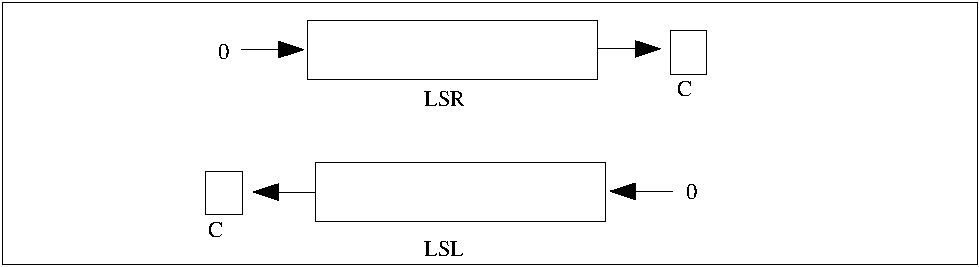
\includegraphics[width=10cm]{graphs/lsrlsl.pdf}
  \caption{Instrucciones de desplazamiento lógico}
  \label{fig:instrSHIFT}
\end{figure}

\begin{figure}[h]
  \centering
    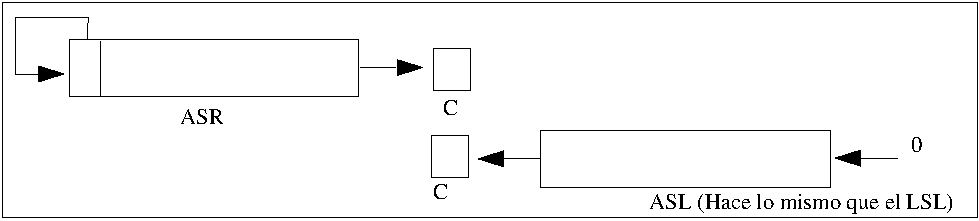
\includegraphics[width=10cm]{graphs/asrasl.pdf}
  \caption{Instrucciones de desplazamiento aritmético}
  \label{fig:instrSHIFTarit}
\end{figure}

Las instrucciones de rotación también desplazan, pero el bit que sale del
valor se realimenta. No existe ninguna instrucción para rotar hacia la
izquierda {\tt ROL}, ya que puede simularse con la de rotación a la derecha
{\tt ROR} que sí existe. En estas instrucciones el bit desplazado fuera
es el mismo que el que entra, además de dejar una copia
en el flag C (figura~\ref{fig:instrRotacion}).

\begin{figure}[h]
  \centering
    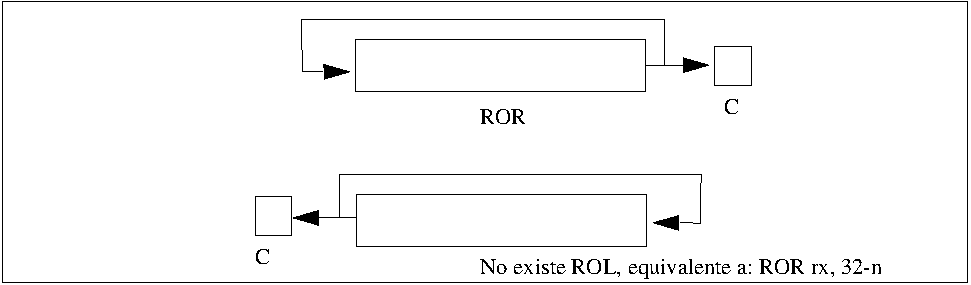
\includegraphics[width=10cm]{graphs/rorrol.pdf}
  \caption{Instrucciones de rotación}
  \label{fig:instrRotacion}
\end{figure}

Las instrucciones de rotación con el carry funcionan de manera
similar, pero el bit que entra es el que había en el flag C y el que sale va a
parar al flag C (figura~\ref{fig:instrRotCarry}). Estas instrucciones
sólo rotan un bit, al contrario que las anteriores que podían rotar/desplazar
varios. La rotación con carry a la derecha es {\tt RRX}, no existe la contrapartida
{\tt RLX} porque se puede sintetizar con otra instrucción ya existente {\tt adcs}.
Con {\tt adcs} podemos sumar un registro consigo mismo, que es lo mismo que multiplicar por 2
o desplazar 1 bit hacia la izquierda. Si a esto le añadimos el bit de carry como entrada
y actualizamos los flags a la salida, tendremos exactamente el mismo comportamiento
que tendría la instrucción {\tt RLX}.

\begin{figure}[h]
  \centering
    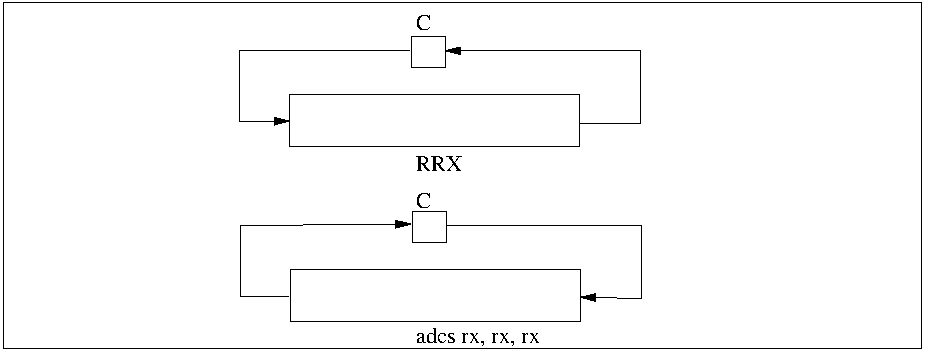
\includegraphics[width=10cm]{graphs/rrxadcs.pdf}
  \caption{Instrucciones de rotación con {\it carry}}
  \label{fig:instrRotCarry}
\end{figure}

También podemos forzar el flag C o cualquier otro flag al
valor que queramos con la siguiente instrucción.

\begin{lstlisting}
        msr     cpsr_f, #valor
\end{lstlisting}

Donde para calcular el valor hacemos el paso inverso al explicado en {\bf gdb}.
Queremos cambiar los flags a estos valores: N=0, Z=1, C=1 y V=0. Por el orden
memorizado de la secuencia {\bf NZCV}, calculamos el nibble binario, que es 0110.
Lo pasamos a hexadecimal 0110 -> 6 y lo ponemos en la parte más alta de la
constante de 32 bits, dejando el resto a cero.

\begin{lstlisting}
        msr     cpsr_f, #0x60000000
\end{lstlisting}

Todas las instrucciones de rotación en realidad son subinstrucciones que el
ensamblador traduce a una instrucción {\bf mov}. Por esa razón las he puesto
en mayúsculas, diferenciándolas de las instrucciones reales que están en
minúscula. En realidad las dos siguientes instrucciones son totalmente
equivalentes.

\begin{lstlisting}
        LSRs    r0, r0, #1
        movs    r0, r0, LSR #1
\end{lstlisting}

Pero se tiende a escoger siempre la más sencilla, en este caso la primera. En
próximas lecciones mostraremos la potencia que tienen las subistrucciones de
desplazamiento/rotación (cuando están en mayúscula mezcladas con los operandos).
Como adelanto, la siguiente instrucción multiplica por 5 el contenido de r0.

\begin{lstlisting}
        add     r0, r0, r0, LSL #2
\end{lstlisting}

\subsubsection{Ejercicio 1.8}
Examina atentamente el programa {\tt intro4.s} (listado \ref{lst:codigoPract4}).
Antes de ejecutarlo completa el siguiente cuadro, después comprueba los resultados con
el {\bf gdb}. Observa la definición de variable {\tt var1: .word 0x80000000}.

\begin{center}
\small
\colorbox[gray]{0.9}{
\tabcolsep = 1mm
\begin{tabular}{c}
\colorbox[gray]{1}{
\begin{tabular}{|p{3cm}||c|c|}
\hline
Instrucción & r1 (binario) & C \\
\hline\hline
ldr r1, [r0]&\rule{6cm}{0cm}&\rule{1cm}{0cm}\\
\hline
LSRs r1, r1, \#1&\rule{6cm}{0cm}&\rule{1cm}{0cm}\\
\hline
LSRs r1, r1, \#3&\rule{6cm}{0cm}&\rule{1cm}{0cm}\\
\hline
\end{tabular}
}
\\[1mm]
\colorbox[gray]{1}{
\begin{tabular}{|p{3cm}||c|c|}
\hline
Instrucción & r2 (binario) & C \\
\hline\hline
ldr r2, [r0]&\rule{6cm}{0cm}&\rule{1cm}{0cm}\\
\hline
ASRs r2, r2, \#1&\rule{6cm}{0cm}&\rule{1cm}{0cm}\\
\hline
ASRs r2, r2, \#3&\rule{6cm}{0cm}&\rule{1cm}{0cm}\\
\hline
\end{tabular}
}
\\[1mm]
\colorbox[gray]{1}{
\begin{tabular}{|p{3cm}||c|c|}
\hline
Instrucción & r3 (binario) & C \\
\hline\hline
ldr r3, [r0]&\rule{6cm}{0cm}&\rule{1cm}{0cm}\\
\hline
RORs r3, r3, \#31&\rule{6cm}{0cm}&\rule{1cm}{0cm}\\
\hline
RORs r3, r3, \#31&\rule{6cm}{0cm}&\rule{1cm}{0cm}\\
\hline
RORs r3, r3, \#24&\rule{6cm}{0cm}&\rule{1cm}{0cm}\\
\hline
\end{tabular}
}
\\[1mm]
\colorbox[gray]{1}{
\begin{tabular}{|p{3.2cm}||c|c|}
\hline
Instrucción & r4 (binario) & C \\
\hline\hline
ldr r4, [r0]&\rule{6cm}{0cm}&\rule{1cm}{0cm}\\
\hline
msr cpsr\_f, \#0&\rule{6cm}{0cm}&\rule{1cm}{0cm}\\
\hline
adcs r4, r4, r4&\rule{6cm}{0cm}&\rule{1cm}{0cm}\\
\hline
adcs r4, r4, r4&\rule{6cm}{0cm}&\rule{1cm}{0cm}\\
\hline
adcs r4, r4, r4&\rule{6cm}{0cm}&\rule{1cm}{0cm}\\
\hline
msr cpsr\_f, \#0x2..&\rule{6cm}{0cm}&\rule{1cm}{0cm}\\
\hline
adcs r4, r4, r4&\rule{6cm}{0cm}&\rule{1cm}{0cm}\\
\hline 
\end{tabular}
}
\\[1mm]
\end{tabular}
}
\end{center}

\begin{lstlisting}[caption={Código del programa intro4.s},label={lst:codigoPract4}]
.data

var1:   .word   0x80000000

.text
.global main

main:   ldr     r0, =var1     /* r0 <- &var1        */
        ldr     r1, [r0]      /* r1 <- *r0          */
        LSRs    r1, r1, #1    /* r1 <- r1 LSR #1    */
        LSRs    r1, r1, #3    /* r1 <- r1 LSR #3    */
        ldr     r2, [r0]      /* r2 <- *r0          */
        ASRs    r2, r2, #1    /* r2 <- r2 ASR #1    */
        ASRs    r2, r2, #3    /* r2 <- r2 ASR #3    */
        ldr     r3, [r0]      /* r3 <- *r0          */
        RORs    r3, r3, #31   /* r3 <- r3 ROL #1    */
        RORs    r3, r3, #31   /* r3 <- r3 ROL #1    */
        RORs    r3, r3, #24   /* r3 <- r3 ROL #8    */
        ldr     r4, [r0]      /* r4 <- *r0          */
        msr     cpsr_f, #0    /* C=0                */
        adcs    r4, r4, r4    /* rotar izda carry   */
        adcs    r4, r4, r4    /* rotar izda carry   */
        adcs    r4, r4, r4    /* rotar izda carry   */
        msr     cpsr_f, #0x20000000 /* C=1          */
        adcs    r4, r4, r4    /* rotar izda carry   */
        bx      lr
\end{lstlisting}

\subsection{Instrucciones de multiplicación}

Las instrucciones de multiplicación admiten muchas posibilidades, debido
a que es una operación en la cual el resultado tiene el doble de bits
que cada operando. En la siguiente tabla vemos las 5 instrucciones de
multiplicación que existen.

\begin{longtable}{| p{2.5cm} | p{2.5cm} | p{7cm} |}
\hline
{\bf Instrucción} & {\bf Bits} & {\bf Nombre} \\ \hline
mul    & 32=32x32 &  Multiplicación truncada \\ \hline
umull  & 64=32x32 & Multiplicación sin signo de 32bits \\ \hline
smull  & 64=32x32 & Multiplicación con signo de 32bits \\ \hline
smulw* & 32=32x16 & Multiplicación con signo de 32x16bits \\ \hline
smul** & 32=16x16 & Multiplicación con signo de 16x16bits \\ \hline
\caption{Instrucciones de multiplicación}
\label{list_mul}
\end{longtable}

La instrucción {\tt mul} realiza una multiplicación truncada, es decir,
nos quedamos con los 32 bits inferiores del resultado. Como el signo
del resultado es el bit más significativo el cual no obtenemos, esta
multiplicación es válida tanto para operandos naturales (sin signo) como
para enteros (con signo). En el ejemplo de abajo {\tt r0 = parte\_baja(r1*r2)}:

\begin{lstlisting}
        mul     r0, r1, r2
\end{lstlisting}

Las dos siguientes multiplicaciones ({\tt umull} y {\tt smull}) son largas,
por eso la {\tt l} del final, donde el resultado es de 64 bits. Si los
operandos son naturales escogemos la multiplicación sin signo (unsigned) {\tt umull}.
Por el contrario, si tenemos dos enteros como factores hablamos de
multiplicación con signo (signed) {\tt smull}. En ambos ejemplos la parte baja del
resultado se almacena en r0, y la parte alta en r1. Para hacer que {\tt r1:r0 = r2*r3}:

\begin{lstlisting}
        umull   r0, r1, r2, r3
        smull   r0, r1, r2, r3
\end{lstlisting}

Ahora veamos {\tt smulw*}. Es con signo, y el asterisco puede ser una {\bf b} para
seleccionar la parte baja del registro del segundo factor, o una {\bf t} para
seleccionar la alta. Según el ejemplo {\tt r0 = r1*parte\_baja(r2)}.

\begin{lstlisting}
        smulwb  r0, r1, r2
\end{lstlisting}

Por último tenemos {\tt smul**} también con signo, donde se seleccionan partes
alta o baja en los dos factores, puesto que ambos son de 16 bits. En el ejemplo
{\tt r0 = parte\_alta(r1)*parte\_baja(r2)}.

\begin{lstlisting}
        smultb  r0, r1, r2
\end{lstlisting}

En los dos últimos tipos {\tt smulw*} y {\tt smul**} no se permite el sufijo {\bf s}
para actualizar los flags.

\subsubsection{Ejercicio 1.9}
Completa los recuadros en blanco con los resultados en hexadecimal empleando
calculadora. Luego ensambla el listado \ref{lst:codigoPract5} y comprueba
mediante {\bf gdb} que los cálculos anteriores son correctos.

\begin{center}
\small
\colorbox[gray]{0.9}{
\tabcolsep = 1mm
\begin{tabular}{cccc}
& Producto & Factor1 & Factor2 \\
mul & 
\colorbox[gray]{1}{\rule{4cm}{0cm}\rule{0cm}{0.46cm}} &
\colorbox[gray]{1}{\rule{2cm}{0cm}\rule{0cm}{0.46cm}} &
\colorbox[gray]{1}{\rule{2cm}{0cm}\rule{0cm}{0.46cm}} \\
umull & 
\colorbox[gray]{1}{\rule{4cm}{0cm}\rule{0cm}{0.46cm}} &
\colorbox[gray]{1}{\rule{2cm}{0cm}\rule{0cm}{0.46cm}} &
\colorbox[gray]{1}{\rule{2cm}{0cm}\rule{0cm}{0.46cm}} \\
smull & 
\colorbox[gray]{1}{\rule{4cm}{0cm}\rule{0cm}{0.46cm}} &
\colorbox[gray]{1}{\rule{2cm}{0cm}\rule{0cm}{0.46cm}} &
\colorbox[gray]{1}{\rule{2cm}{0cm}\rule{0cm}{0.46cm}} \\
smuwb & 
\colorbox[gray]{1}{\rule{4cm}{0cm}\rule{0cm}{0.46cm}} &
\colorbox[gray]{1}{\rule{2cm}{0cm}\rule{0cm}{0.46cm}} &
\colorbox[gray]{1}{\rule{2cm}{0cm}\rule{0cm}{0.46cm}} \\
smutt & 
\colorbox[gray]{1}{\rule{4cm}{0cm}\rule{0cm}{0.46cm}} &
\colorbox[gray]{1}{\rule{2cm}{0cm}\rule{0cm}{0.46cm}} &
\colorbox[gray]{1}{\rule{2cm}{0cm}\rule{0cm}{0.46cm}} \\
\end{tabular}
}
\end{center}

\begin{lstlisting}[caption={Código del programa intro5.s},label={lst:codigoPract5}]
.data
var1:   .word   0x12345678
var2:   .word   0x87654321
var3:   .word   0x00012345

.text
.global main
main:   ldr     r0, =var1         /* r0 <- &var1        */
        ldr     r1, =var2         /* r1 <- &var2        */
        ldr     r2, =var3         /* r2 <- &var3        */
        ldrh    r3, [r0]          /* r3 <- baja(*r0)    */
        ldrh    r4, [r1]          /* r4 <- baja(*r1)    */
        muls    r5, r3, r4        /* r5 <- r3*r4        */
        ldr     r3, [r0]          /* r3 <- *r0          */
        ldr     r4, [r1]          /* r4 <- *r1          */
        umull   r5, r6, r3, r4    /* r6:r5 <- r3*r4     */
        smull   r5, r6, r3, r4    /* r6:r5 <- r3*r4     */
        ldrh    r3, [r0]          /* r3 <- baja(*r0)    */
        ldr     r4, [r2]          /* r4 <- *r2          */
        smulwb  r5, r3, r4        /* r5 <- r3*baja(r4)  */
        smultt  r5, r3, r4    /* r5 <- alta(r3)*alta(r4)*/
\end{lstlisting}



\chapterend{}
